\documentclass[tikz]{standalone}

% Font
\usepackage{mathpazo}
\usepackage{libertine}
\renewcommand*\sfdefault{phv}

\large

% Color
\usepackage{xcolor}
\definecolor{f1}{HTML}{F39019}
\definecolor{b1}{HTML}{DE6A10}
\definecolor{f2}{HTML}{51A7F9}
\definecolor{b2}{HTML}{0365C0}
\definecolor{f3}{HTML}{70BF41}
\definecolor{b3}{HTML}{00882B}

% tikz
\usepackage{tikz}
\tikzstyle{every node}=[font=\sffamily]
\usetikzlibrary{shapes,arrows,positioning,calc,decorations.markings,backgrounds}
\tikzstyle{c1} = [thick,draw=b1,fill=f1]
\tikzstyle{c2} = [thick,draw=b2,fill=f2]
\tikzstyle{c3} = [thick,draw=b3,fill=f3]
\tikzstyle{cg} = [thick,draw=gray!50,fill=gray!30]
\tikzstyle{rect} = [rectangle, minimum height=1cm]
\tikzstyle{roundrect} = [rect, rounded corners=.2cm]
\tikzstyle{io} = [trapezium, trapezium left angle=70, trapezium right angle=110]
\tikzstyle{arrow} = [thick,->,>=stealth]

\tikzstyle{box} = [draw=gray, very thick, text width=5.6cm, align=center]
\tikzstyle{title} = [font=\bfseries \rmfamily \large, anchor=north west]

\begin{document}
	
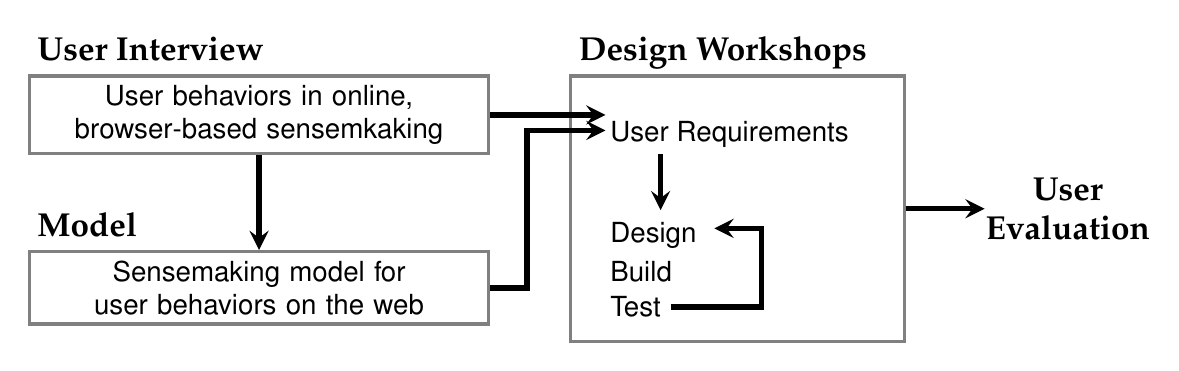
\begin{tikzpicture}
\node (interview) [box] {User behaviors in online, browser-based sensemkaking};
\node (interview-text) [above=.6 of interview.north west, title] {User Interview};

\node (model) [box, below=1.2 of interview] {Sensemaking model for user behaviors on the web};
\node (model-text) [above=.6 of model.north west, title] {Model};
\draw [arrow, line width=2pt] (interview) -- (model);

\node (design) [box, right=1 of interview.north east, anchor=north west, minimum height=3.37cm, text width=4cm] {};
\node (design-text) [above=.6 of design.north west, title] {Design Workshops};
\node (req) [below=0.47 of design.north west, anchor=north west, xshift=.4cm] {User Requirements};
\draw [arrow, line width=2pt] (interview) --++(4.4,0);
\draw [arrow, line width=2pt] (model) -|++(3.4,2) --++(1,0);

\node (des) [below= of req.west, anchor=north west] {Design};
\node (build) [below= .2 of des.west, anchor=north west] {Build};
\node (test) [below= .2 of build.west, anchor=north west] {Test};
\draw [arrow, line width=2pt] (test) -|++(1.6,1) --++ (-.6,0);
\draw [arrow, line width=2pt] (5.1,-.5) --++ (0,-.71);

\node (eval) [title, right=of design, text width=2.1cm, align=center, inner sep=0] {User Evaluation};
\draw [arrow, line width=2pt] (design) -- (eval);

\end{tikzpicture}
	
\end{document}